\documentclass{article}
\usepackage{amsmath,mathtools}
\usepackage{amssymb}
\usepackage{float}
\usepackage{url}
\usepackage[dvipsnames]{xcolor}
\usepackage{graphicx}
\usepackage{tikz}
\usepackage{float}
\usepackage{subcaption}
\usepackage{pgfplots}
\usetikzlibrary{arrows}
\usetikzlibrary{datavisualization.formats.functions}
\usepgfplotslibrary{fillbetween}
\usetikzlibrary{patterns}
\usepackage{xargs}
\usepackage{enumitem}
\usepackage{systeme}
\usepackage{centernot}
\usepackage{algpseudocode}
\usepackage{physics}
\usepackage{xfrac}
\usepackage{titling}
\usepackage[top=.75in, bottom=.75in, left=1in, right=1in]{geometry}
\usepackage[skins,theorems]{tcolorbox}
\tcbset{highlight math style={enhanced,
  colframe=blue,colback=white,arc=0pt,boxrule=1pt}}

% calculus commands
\renewcommand{\eval}[3]{\left[#1\right]_{#2}^{#3}}

% linear algebra commands
\newcommand{\icol}[1]{% inline column vector
  \begin{bsmallmatrix}#1\end{bsmallmatrix}%
}
\renewcommand\vec{\mathbf}
\newenvironment{sysmatrix}[1]
{\left[\begin{array}{@{}#1@{}}}
{\end{array}\right]}
\newcommand{\ro}[1]{%
\xrightarrow{\mathmakebox[\rowidth]{#1}}%
}
\newlength{\rowidth}% row operation width
\AtBeginDocument{\setlength{\rowidth}{3em}}

%set theory commands
\newcommand{\pset}[1]{\mathcal P(#1)}
\newcommand{\card}[1]{\operatorname{card}(#1)}
\newcommand{\R}{\mathbb R}

%optimization commands
\DeclareMathOperator*{\argmax}{arg\,max}
\DeclareMathOperator*{\argmin}{arg\,min}

%misc commands
\newcommand*\circled[1]{\tikz[baseline=(char.base)]{
             \node[shape=circle,draw,inner sep=2pt] (char) {#1};}}

\let\oldabstract\abstract
\let\oldendabstract\endabstract
\makeatletter
\renewenvironment{abstract}
{\renewenvironment{quotation}%
  {\list{}{\addtolength{\leftmargin}{6em} % change this value to add or remove length to the the default
      \listparindent 1.5em%
      \itemindent    \listparindent%
      \rightmargin   \leftmargin%
      \parsep        \z@ \@plus\p@}%
    \item\relax}%
  {\endlist}%
\oldabstract}
{\oldendabstract}
\makeatother

\setlength{\droptitle}{-7em}   % This is your set screw

\begin{document}

\title{On Gradient Descent\\and its Variants}
\author{Ozaner Hansha}
\date{April 12, 2021}
\maketitle

\begin{abstract}
    We examine the gradient descent (GD) algorithm, with respect to arbitrary real functions $f:\R^n\to\R$. In particular, we elaborate on its formulation, complexity, and convergence conditions. We then introduce and do the same with two variants of GD, namely stochastic gradient descent (SGD) and Adam.
\end{abstract}

\section*{Background}
First developed by French mathematician Cauchy in 1847 \cite{cauchyAndGradient}, \textbf{gradient descent} (GD) is an iterative optimization algorithm used to find a minimum, specifically a \textit{local} minimum, of a multivariate real function. GD has become more prominent recently due to its use in optimizing machine learning models, which have become particularly useful in the last decade or so. It is for this very reason that stochastic gradient descent, a modification of GD, is often cited as `the workhorse of machine learning.'

And so, in an effort to better inform the usage of this algorithm, this paper will attempt to provide both a intuitive and mathematical basis for GD. We then consider how this basis changes, if at all, when considering two of GD's modern incarnations: stochastic gradient descent (SGD), and Adam.

\section*{Gradient Descent}
\subsection*{Overview}
  Before we dive into the formulation of GD, let us first get an intuitive view of how the algorithm works. Consider a function $f(x_1,x_2)$ which we wish to minimize. This function takes two parameters, and so we can represent it via the following 3D plot:

  \begin{figure}[h]
    \centering
    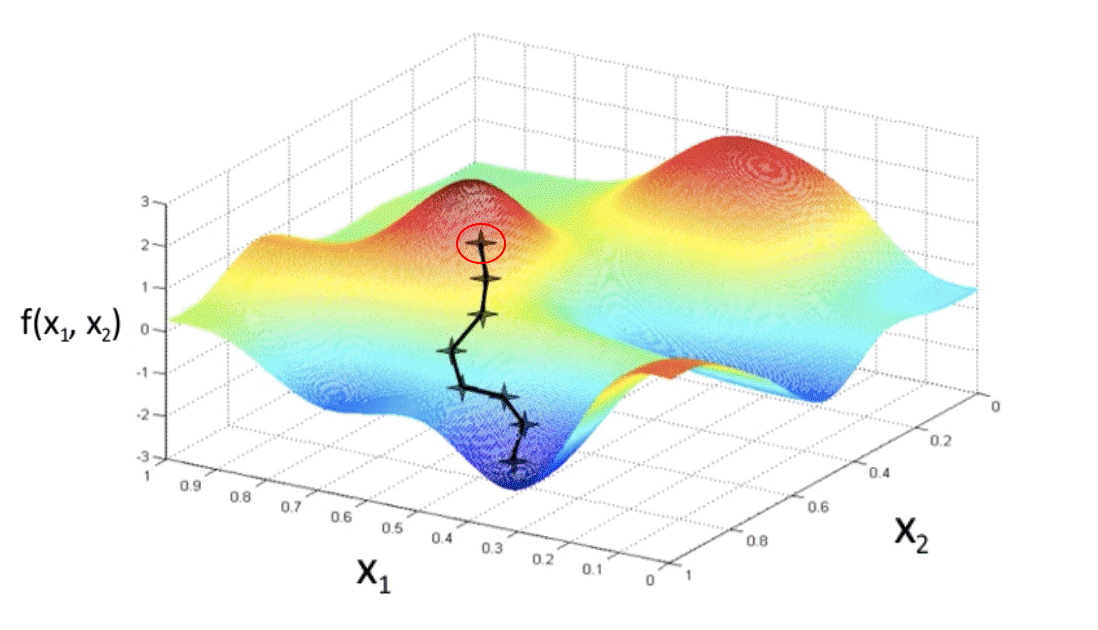
\includegraphics[scale=.5]{hill}
    \caption{An arbitrary 2D surface. Red-Blue $\iff$ High-Low.}
  \end{figure}

  With this setup, we can now describe the GD algorithm in geometric terms. Given some initial guess, here circled in red, GD prescribes:
  \begin{enumerate}
    \item At the point you are on, find the direction which slopes downwards the most. 
    \item Step down this direction a small amount.
    \item Repeat 1 \& 2 until there is no direction which slopes downards at our position.
  \end{enumerate}

  We can picture this like rolling a ball down a hill, sans the momentum. The ball will keep rolling down the hill until it reaches a valley which, in this case, is our minimum. Note however that the minimum our point/ball ends up in is not necessarily the global minimum, just a local one. After all, there may always be a lower valley to reach if we could travel uphill slightly more, as in this 2D example:

  \begin{figure}[h]
    \centering
    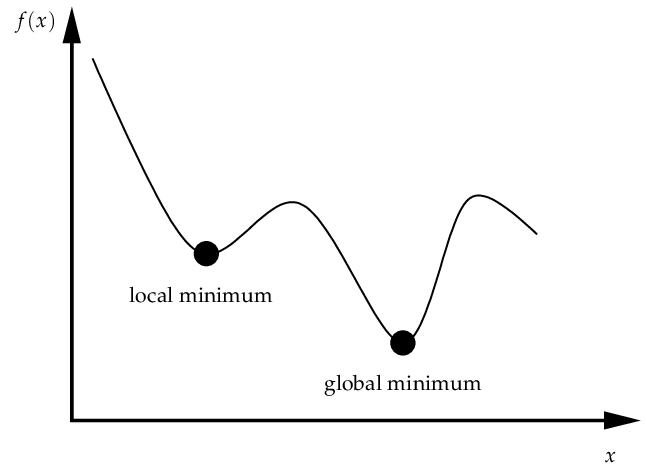
\includegraphics[scale=.45]{local}
    \caption{An arbitrary 1D surface.}
  \end{figure}

  Note that this property of GD of only considering its immediate surroundings and potentially missing out on a global minimum is called \textbf{greediness}. While such a property may not seem desirable, it is impossible, at least in general, to consider an entire function at once to ascertain its minimum. If it was, the problem of optimization wouldn't be much of a problem at all!

\subsection*{Formulation}
  Now let us convert the intuitive description of the algorithm given above into a mathematical one. We'll start by first laying out the algorithm:
  \vspace{5mm}

  \begin{algorithmic}
    \Function{GradientDescent}{$f,\gamma,iter$}
    \State $\vec x_0\gets$ initial value
    \For{$i\in\{1,2,\cdots,iter\}$}
      \State $\vec x_i\gets\vec x_{i-1} - \gamma\nabla f(\vec x_{i-1})$
    \EndFor
    \State \Return $\vec x_{iter}$
  \EndFunction
  \end{algorithmic}
  \vspace{5mm}

  Our goal is to minimize $f:\R^n\to\R$, an $n$ dimensional multivariate function. You'll note that in formulating GD mathematically, we have generalized it to $n>3$. That said, while it is intuitive that GD works for $n=2,3$ (e.g. a ball rolling down a hill) and while the algorithm is no different in higher dimensions, we should still be dubious that it is \textit{effective} for $n>3$. This is a point we will confirm, at least partially, in the section on convergence.

  The algorithm has us start with an initial value $\vec x_0$, analogous to the ball's starting position in the hill example. It would be ideal to set this to an educated guess, but often we have no idea where the minimum will be before hand. As such, for practical usage, it is common to set it to some random vector near the origin, although a more appropriate choice would depend on the function $f$.

  Once this initial value is set, we compute the gradient of $f$ at $\vec x_0$, multiply it by some small value $\gamma$, then subtract it from $\vec x_0$ to produce a new, usually smaller, $\vec x_1$. Note that the usage of the gradient of $f$ means that GD demands that $f$ be differentiable, although with slight modification sub-differentiability may suffice.
  
  The gradient here is analogous to the `direction that slopes downward the most' in the hill example, while $\gamma$ is analogous to how big the steps we take are in said direction. We often set $\gamma$ to be some small value. If the steps are too big, we might overstep the minimum, and if they were \textit{too} small we'd waste computing time with all the extra iterations:

  \begin{figure}[H]
    \centering
    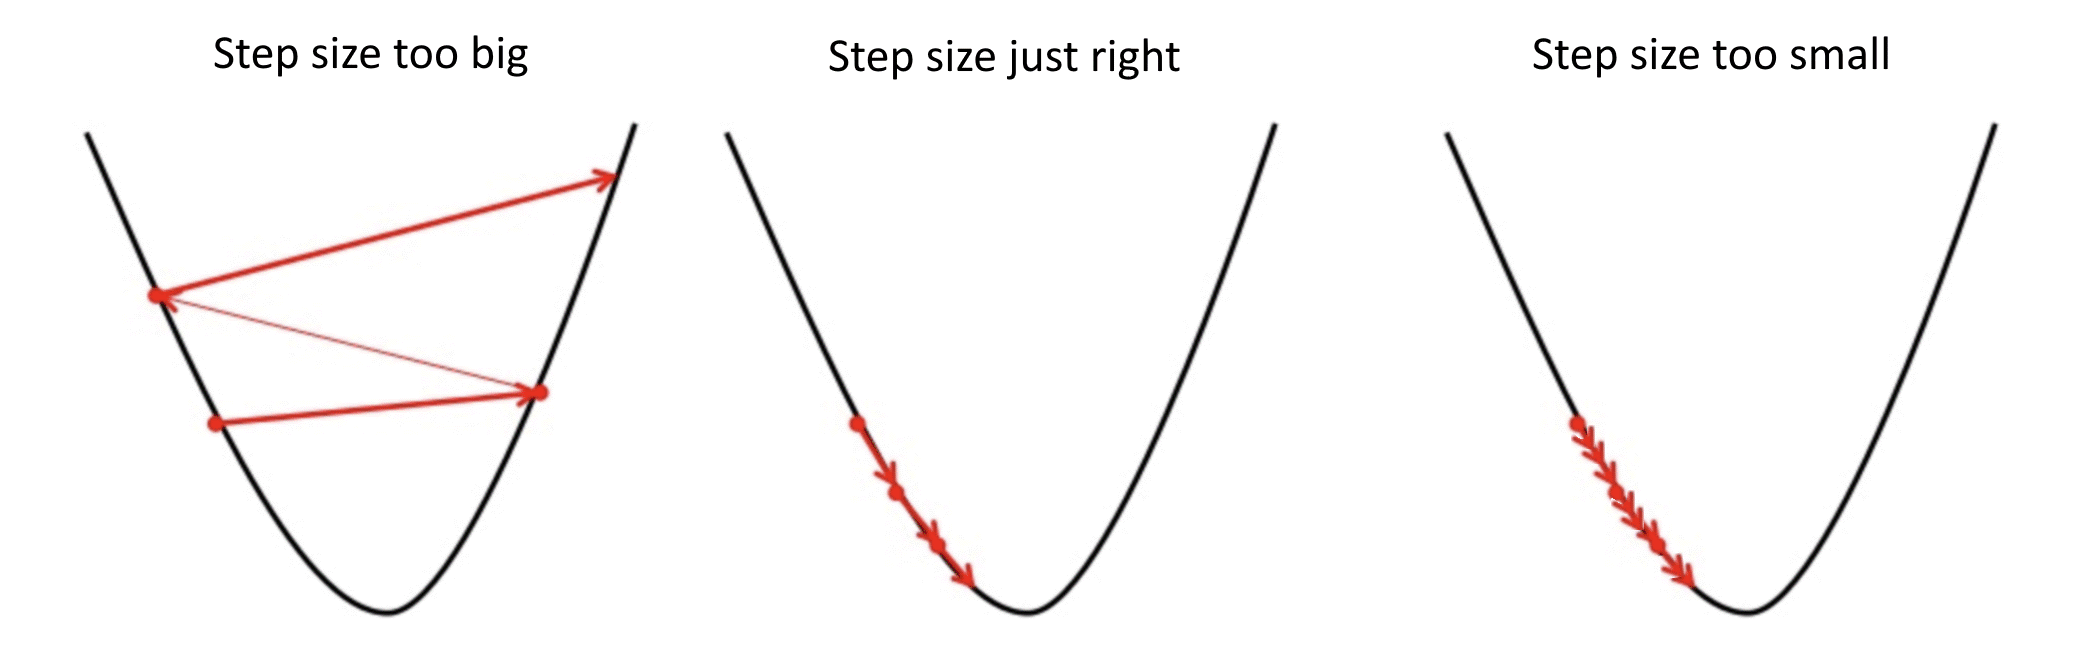
\includegraphics[scale=.3]{stepsize}
    \caption{The problem with extreme step sizes.}
  \end{figure}

  But `small' is relative, and so we must take care to scale $\gamma$ appropriately to $f$ or vice versa. There are also more structured ways of choosing values for $\gamma$ such as scheduling, where the value of $\gamma$ changes every iteration. An example of this is a linear schedule, where $\gamma_i$ decreases by some fixed amount every iteration. A full discussion of these methods are beyond the scope of this paper however.

  Getting back to the algorithm, after $\vec x_1$ is computed, the process is repeated to calculate $\vec x_2$ and so on $iter$ times. It is at this point that our algorithm is finished and returns our result: $\vec x_{iter}$. How do we decide on $iter$? Again the most appropriate value depends on the problem. Often, instead of a set number of iterations, GD's stopping condition is whether $\|\vec x_i-\vec x_{i-1}\|<\delta$ for some small, predetermined value of $\delta$. This condition signals that $\vec x_i$ has converged and that more iterations are unnecessary. When this stopping condition is used, it is often coupled by having a variable $maxiter$ represent the maximum number of iterations GD can take before giving up. We can reprhase GD, then, as \cite{2016arXiv160904747R}:
  \vspace{5mm}picked

  \begin{algorithmic}
    \Function{GradientDescent}{$f,\gamma,\delta,maxiter$}
    \State $\vec x_0\gets$ initial value
    \For{$i\in\{1,2,\cdots,maxiter\}$}
      \State $\vec x_i\gets\vec x_{i-1} - \gamma\nabla f(\vec x_{i-1})$
      \If{$||\vec x_i-\vec x_{i-1}\|<\delta$}
        \State \Return $\vec x_i$
      \EndIf
    \EndFor
    \State \Return $\vec x_{maxiter}$
  \EndFunction
  \end{algorithmic}

\subsection*{Complexity}
  In the worst case scenario, our GD algorithm takes $k=maxiter$ iterations to return a result. As such, the worst case time complexity of GD is $O(k)$ right? Well, this ignores the time taken to compute the gradient of $f$ with respect to some $\vec x_i$. Indeed, while we've written this as a single step in the previous section, it will take at least $n$ steps, one for each component of the gradient. Since all $n$ of these components need to be computed for each iteration, our final worst-case temporal complexity is:
  $$O(k^2n)\qquad\substack{\text{assuming the time to compute $\dv{f}{x_i}$}\\\text{doesn't depend on $n$.}}$$

  In other words, the time taken has a quadratic relationship with number of iterations of GD, and a linear relationship with dimensionality of the function being minimized. 

  In terms of spatial complexity, i.e. how much storage is needed to run GD, we only need to store our current point (or the current point AND the last point if we use the convergence criterion), and whatever storage is needed to store/compute the gradient. Since there are $n$ components to these vectors, our spatial complexity is simply:
  $$O(n)$$
  
\subsection*{Convergence}
  While we cannot demonstrate all functions which converge under GD, we can highlight an important subclass of them. Let our function $f$ be convex and differentiable, with $\nabla f$ Lipschitz continuous, meaning:
  $$\exists L>0,\forall x,y,\quad\|\nabla f(\vec x)-\nabla f(\vec y)\|\le L\|x-y\|$$

  Then if we run GD for $k$ iterations with a fixed step size $\gamma\le 1/L$, then we have:
  $$f(\vec x_k)-f(\vec x^*)\le\frac{\|\vec x_0-\vec x^*\|^2}{2k\gamma}$$

  Where $\vec x^*$ achieves the minimum of $f$. This result means that, under the given conditions, GD is guaranteed to converge and with a rate at least proportional to $1/k$ \cite{tibshirani_2013}.

\section*{Stochastic Gradient Descent}
\subsection*{GD's Computational Burden}
As mentioned previously, GD is often used in fitting machine learning models. In these cases, we are trying to find $n$ parameters $\boldsymbol\omega$ that minimize the error our model $M_{\boldsymbol\omega}:X\to Y$ produces with some dataset $D=\{(\vec x_i,y_i)\mid i\in[1..S]\}$ with $S$ samples. Using the mean square error (MSE), our function $f$ would look something like this:
$$f(\boldsymbol\omega)=\frac{1}{S}\sum^{S}_{i=1} (M_{\boldsymbol\omega}(\vec x_i)-y_i)^2$$

Note that the closer the model's predictions of $\vec x_i$ are to the real answers $y_i$, the lower $f$ is. Indeed if there are no errors we expect to see $f$ reach 0. It seems, then, that minimizing $f$ is a reasonable approach to achieving parameters $\boldsymbol\omega$ for a more accurate model $M_{\boldsymbol\omega}$, assuming doing better on this training set $D$ produces a better model.

This problem forms the backbone of modern machine learning, which often boils down to finding optimal parameters of very complex models. However, there is a problem. In real world data sets, the size $S$ is often enormous. Possibly on the order of millions. Computing $\nabla f$ for each iteration of gradient descent can be prohibitively time consuming. This is because the number of components $n$ of $\boldsymbol\omega$ (i.e. the number of parameters in the model) can go into the hundreds.

\subsection*{Mini-batch Gradient Descent}
Since computing the gradient for each of the potentially millions of training examples is burdensome to do for each iteration of GD, we could simply look at less of the data set at a time. One approach to leverage this intuition is the following:
\begin{enumerate}
  \item Partition the data set $D$ into $p$ equally sized subsets $\{D_i\}_{i=1}^p$, each called a \textbf{mini-batch}.
  \item For each mini-batch $i$:
  \begin{enumerate}
    \item Run GD on a modified function $f_i$ defined as:
    $$f_i(\boldsymbol\omega)=\frac{1}{|D_i|}\sum_{(\vec x,y)\in D_i} (M_{\boldsymbol\omega}(\vec x)-y)^2$$
    \item Update $\boldsymbol\omega$ to the result of this GD.
  \end{enumerate}
  \item After all mini-batches, we arrive at our final $\boldsymbol\omega$, and can repeat step 2 more times if necessary.
\end{enumerate}

This method, aptly dubbed \textbf{mini-batch gradient descent} \cite{2019arXiv190303614Z}, has the advantage of not having to compute $\nabla f$ for every single training example before some progress can be made in moving towards the minimum. More progress made down the gradient speeds up later iterations. The trade-off is that the calculation of the gradient at each mini-batch is no longer exact, but an approximation using only some of the data. In other words, our algorithm was made a bit more noisy. In order to minimize this trade-off, we must make sure the examples in our mini-batches are randomly distributed so as to be representative of the entire dataset.

All that said, this trade-off is usually well worth due to the time savings. Indeed, with said time savings, one could just run more iterations of this mini-batch GD, and/or even subdivide the dataset further\dots

\subsection*{Stochastic GD}
Taking the mini-batch approach to the extreme, we could have mini-batches of size 1, effectively computing updating our parameters $\boldsymbol\omega$ for each datapoint $d\in D$. This is called \textbf{stochastic gradient descent} (SGD) \cite{2019arXiv190303614Z}. Below we demonstrate the SGD algorithm:
\vspace{5mm}

\begin{algorithmic}
  \Function{StochasticGD}{$\gamma,\delta,maxiter$}
  \State $\boldsymbol\omega_0\gets$ initial value
  \State $i\gets 1$
  \Repeat
    \State Pick random $(\vec x, y)\in D$
    \State $\boldsymbol\omega_i\gets\boldsymbol\omega_{i-1}-\gamma\nabla(M_{\omega_{i-1}}(\vec x)-y)^2$
    $i\gets i+1$
  \Until{$\boldsymbol\omega_i-\boldsymbol\omega_{i-1} < \delta \vee i > maxiter$}
  \State \Return $\boldsymbol\omega_i$
\EndFunction
\end{algorithmic}
\vspace{5mm}

Here we simply pick a random datapoint $d\in D$, slightly adjust our parameter values $\boldsymbol\omega$ based on the gradient we calculate with $d$, and repeat until we converge or just hit our iteration limit. While noisy, as it only calculates an approximate gradient, SGD has the benefit of immediate feeback for the model parameters, making learning quick. And as long as the datapoints uniformly random (and thus representative of the dataset) and enough iterations are run, the parmeters should converge just as well as they did with GD, just in a faster and slightly less precise manner.

\section*{Momentum based methods}
While there many variants of GD, specifically of SGD, most of them make use of momentum \cite{2016arXiv160904747R}. To see what this means, consider the ball on a hill example we made use of previously. The example was a little flawed as the ball/point/parameters GD keeps track of doesn't have momentum. It just travels down the hill/gradient at a constant speed, determined by the step-size $\gamma$.

A ball in real life, however, would accrue some momentum from falling down a hill, meaning it would not follow the steepest path down a hill but some combination of that steepest path and whatever direction the ball has momentum in. Such a property would allow the ball to clear small hills that may be in the way to lower points on the hill:

\begin{figure}[H]
  \centering
  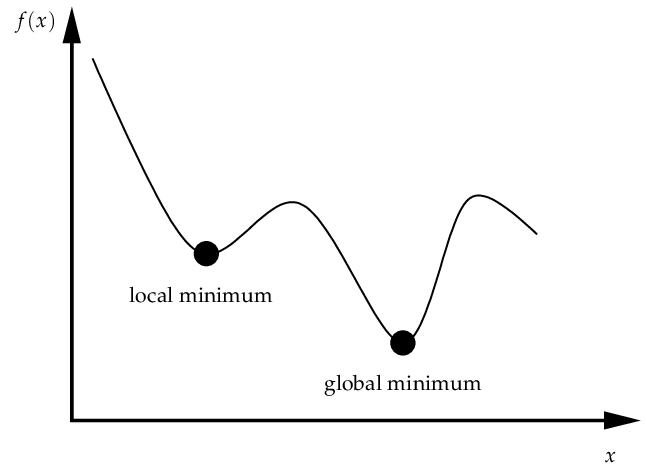
\includegraphics[scale=.45]{local}
\end{figure}

Thus, keeping track of the ball's, or rather, the point's momentum (or some equivalent of it) might serve useful in creating a GD variant that is resistant to bumps in the high dimensional surface $f$ defines. One way this is done is modifying the parmeter update formula:

$$\boldsymbol\omega\rightarrow\boldsymbol\omega-\gamma\nabla f(\boldsymbol\omega)+\alpha\Delta\boldsymbol\omega$$

Where $f(\boldsymbol\omega)$ is the function we seek to minimize, $\gamma$ is the step-size, $\Delta\boldsymbol\omega$ is the change made during last update, and $\alpha$ is how much weight we should put towards that last update. The greater $\alpha$ is, the more the momentum of the parameters comes into play. We can think of it as analogous to the strength of gravity on the ball. We can also apply a schedule to it, just as with $\gamma$, so that its influence diminishess as our paremeters become more and more fine-tuned.

% \section*{Adam}
% \subsection*{Overview}
% Intro what's changed and why it was changed. Maybe a nice graphic.

% Same sections are before, but shorted since even less needs to be introduced and mostly focuses on what's changed.\cite{2019arXiv190303614Z} \cite{2016arXiv160904747R}

\bibliographystyle{plain}
\bibliography{bib2}

\end{document}